\section{Building the scheduler from the modules}\label{sec:compiler}

To prove Theorem~\ref{thm:scheduler}, assign one module to each request of the client.
At a probe, a ready module either supplies a tight quick output or passes the test to
every child attached at a single price (Lemma~\ref{lem:descent}). A restriction may
also leave the module short of a coordinate. In that case viability of the scheduler
program provides an upgrade at the request for the missing coordinate. We now build a
client signature that permits both continuations and show that the tight outputs at
any vertex certify a viable set of client requests.

\subsection{Assigning modules and coordinates}

The recursive construction has three parameters. The module height is \(t\).
Coordinates shared by all buckets are requested in a \emph{common bank} of signature
\(T_0\). Coordinates specific to bucket \(P\) are requested in its \emph{terminal
bank}, of signature \(T_1\) for every \(P\). Write \(\mathcal T(t,T_0,T_1)\) for
the signature we build from these parameters. For the scheduler on \(T\) we take
\[
                     T^+=\mathcal T(h,T,T).
\]
At the initial call the root bank on \(T\) serves in all bank roles. Even when two
roles use the same bank, each new request has its own identity and successor banks.

A direct client request receives a module of height \(t\). For \(t>0\), request the
\(2V\) coordinates associated to \(W_\ell,p_\ell\) in the common bank and the
\(2V\) coordinates associated to \(F_{\ell,P},G_{\ell,P}\) in the terminal bank of
each \(P\). These are the individual blocking coordinates of
\eqref{eq:module-coordinates}. At \(t=0\) request only the single output coordinate
in each terminal bank.

The following options define the successor signatures of \(\mathcal T(t,T_0,T_1)\)
and the attachment of the modules for their client programs. In each case an empty
program creates no modules.
\begin{enumerate}
\item \emph{Price.} At positive height, label \(\ell\) gives an option with signature
\(\mathcal T(t-1,T_0,T_1)\). Keep the banks and attach the roots of this new call at
label \(\ell\) of the present module.
\item \emph{Common bank.} Choose one common position and an option \(\alpha\) of
\(T_0\). Replace the common bank by the \(\alpha\)-successor bank of the request in
that position. With \((T_0)_\alpha\) denoting the corresponding successor signature,
the new call has signature \(\mathcal T(t,(T_0)_\alpha,T_1)\).
\item \emph{Terminal banks.} Choose one terminal position name and an option \(\beta\)
of \(T_1\). For every bucket \(P\), take the \(\beta\)-successor bank of the request
in that position of \(P\). The signature is \(\mathcal T(t,T_0,(T_1)_\beta)\).
For example, the name \(F_\ell\) denotes position \(F_{\ell,P}\) in each terminal
bank. One choice of name and option works simultaneously for all buckets.
\end{enumerate}
For either bank option the roots of the new call have the same incoming physical
attachment as the present module. At the top of the forest they are themselves
physical roots. Calls using the same scheduler bank concatenate their direct requests
there and preserve the successor banks of each request. This gives a program on \(T\).
Figure~\ref{fig:request-upgrades} shows the two physical attachments. In a price
upgrade all the attached outputs use the same \(p_\ell\), hence the same two blocking
coordinates for that price.

\begin{figure}[htbp]
\centering
\definecolor{moduleink}{RGB}{40,82,94}
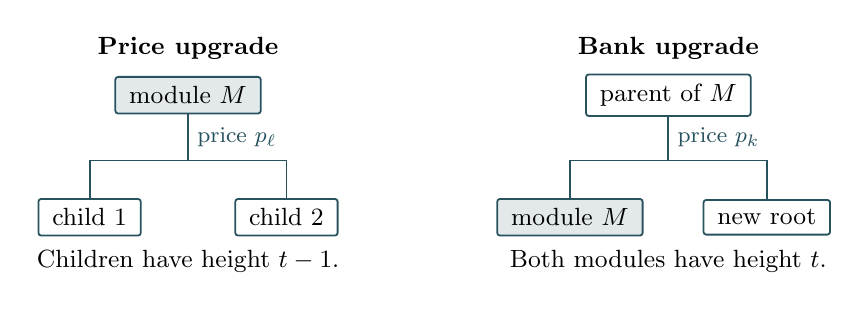
\begin{tikzpicture}[x=1cm,y=1cm,font=\small,line width=.65pt,
  module/.style={draw=moduleink,rounded corners=1pt,inner xsep=5pt,inner ysep=3.5pt},
  current/.style={module,fill=moduleink!13},edge/.style={draw=moduleink},
  linklabel/.style={font=\footnotesize,text=moduleink,fill=white,inner sep=1.3pt}]
  \node at (0,2.15) {\textbf{Price upgrade}};
  \node[current] (m) at (0,1.55) {module \(M\)};
  \node[module] (c1) at (-1.25,0) {child \(1\)};
  \node[module] (c2) at (1.25,0) {child \(2\)};
  \draw[edge] (m.south) -- (0,.72) -- (-1.25,.72) -- (c1.north);
  \draw[edge] (0,.72) -- (1.25,.72) -- (c2.north);
  \node[linklabel,anchor=west] at (.06,1.02) {price \(p_\ell\)};
  \node at (0,-.56) {Children have height \(t-1\).};
  \begin{scope}[shift={(6.1,0)}]
    \node at (0,2.15) {\textbf{Bank upgrade}};
    \node[module] (up) at (0,1.55) {parent of \(M\)};
    \node[current] (old) at (-1.25,0) {module \(M\)};
    \node[module] (new) at (1.25,0) {new root};
    \draw[edge] (up.south) -- (0,.72) -- (-1.25,.72) -- (old.north);
    \draw[edge] (0,.72) -- (1.25,.72) -- (new.north);
    \node[linklabel,anchor=west] at (.06,1.02) {price \(p_k\)};
    \node at (0,-.56) {Both modules have height \(t\).};
  \end{scope}
\end{tikzpicture}
\caption{The two physical attachments for an upgrade at module \(M\) of
height \(t\). At a price upgrade, child outputs \(v_1,v_2\) reach \(M\)
as \(p_\ell+\varepsilon v_1\) and \(p_\ell+\varepsilon v_2\).
A bank upgrade places its new roots alongside \(M\), at the same incoming
price \(p_k\) when \(M\) has a parent.}
\label{fig:request-upgrades}
\end{figure}


Along any option path \(t\) decreases at most \(h\) times. Each bank signature also
descends at most \(H\) times. Thus \(T^+\) has height at most \(h+2H\). If \(G\)
bounds the outdegree in \(T\), a positive-height call has at most \(V+4VG\) options,
and a height-zero call has at most \(G\). In particular the signature is independent
of \(B\), the client program and the sample times. For \(m\) client requests the
forest has \(m\) modules. The number of scheduler coordinates per module is
\(2V+2VB\le4VB\) at positive height and \(B\) at height zero.

Build the physical inequalities as in Section~\ref{sec:layers}. Declare the floors
on all root outputs \emph{red}. Each is a single affine row because the shift is zero
at the root. Propagating a quick output along its physical ancestors produces a
unique root output, preserving the bucket and the originating request. This gives
the groups of red rows indexed by \((P,i)\). A group contains one row for a height-zero
module and \(2V\) rows for a positive-height module. The bounds on \(W\), the links
and the height-zero time bounds supply individual lower bounds on all coordinates
after deleting the red rows.

\subsection{Viability at probes and separation at anchors}

Fix a probe of \(P\) and a coordinate restriction viable for the scheduler.
Independently raise the retained red floors within their allowances from
Lemma~\ref{lem:descent}, and take any vertex of the resulting slice. Declare \(i\)
usable for the client when a retained red row in group \((P,i)\) is tight there.

At each call we maintain two facts. First, the common bank and the terminal bank
of \(P\) have viable programs, including requests placed there by other calls.
Second, at each physical root of this call's forest, the point in its subtree is
a vertex under permitted raises of its retained output floors. Whenever one of
these floors is tight in bucket \(P\), its propagated red row is tight at the
original vertex. At the initial call the banks coincide and the restricted slice
is a product over its physical roots. Both facts therefore hold.

Consider a direct client request of the call. If its module is missing a coordinate
required for readiness, the scheduler restriction omits the request in that position.
Its bank is viable, so an option at the omitted request leads to a viable successor
bank. Take the corresponding bank option of the client. The unchanged bank stays
viable, and the new call's physical roots already belong to the present call's
forest of roots. Both facts pass to this option. For a terminal-bank upgrade we need
viability of the new terminal bank only for the probed \(P\).

For a ready module, a tight quick floor in \(P\) makes the direct client request
usable by the second fact. Otherwise Lemma~\ref{lem:descent} selects a price.
Every child at that label inherits a vertex, and every tight child floor propagates
to the parent. The price option therefore inherits both facts, also when it has no
children. Induction on the remaining signature height proves that each direct
request is usable or has a viable upgrade. This proves the required viability
at the probe for all allowed raises.

At an anchor the unraised red floors have value zero. Distinct outputs in a single
class have a strictly positive lower bound on their sum. Take the raises, the later
perturbations of rows and the tolerances for small violations and near equalities
all sufficiently small compared with the least of these pair gaps. Two nearly
tight outputs in the same class would then violate their pair row beyond the
tolerance. Each class accounts for at most one bucket. There are at most \(2Vm\)
classes, giving the anchor bound. When \(B=1\) the conclusion is immediate.

\subsection{Reducing the number of rows}

Only the slices at the prescribed probes and anchors enter the preceding arguments.
We use this to choose enough affine pieces to preserve those slices. The probe
bands will follow by perturbation.

At each of the \(N(B+2)\) probe and anchor times, choose the time block containing
this sample at each module's height. For every ordinary bound in the block,
including its tournament constraints, keep one affine piece attaining the bound
at the sample. For the coarse bounds do this for each inequality
\eqref{eq:coarse-rows} generated \emph{at} the sample. Take the union of these
rows, all root red and pair rows, and one surviving individual lower bound for
every coordinate after red deletion.

At any selected sample, the retained coarse inequalities give exactly the required
membership \eqref{eq:layer-state}. The strict supporting-line bounds of
Section~\ref{sec:layers} then give all coarse inequalities from other samples of
the same block. The chosen ordinary pieces realize their full bounds there.
Starting with the leaves, block dominance at a module now gives the inequalities
of every other block at its height once its descendants satisfy their full systems.
Consequently the pruned and full slices agree at every probe and anchor. This
agreement persists after raising the red floors, all of which were retained. Both
blocking systems project exactly onto each coordinate restriction. On those slices
the vertex sets and the identities of tight red rows thus also agree.

A module has at most \(2VBm\) outputs, including all those propagated from its
descendants. The pairs of outputs contribute \(O_{r,L,V}((Bm)^2)\) ordinary bounds
in its current block. Its other ordinary bounds, including all label tuples over
\(L\) sites, fit in \(O_{r,L,V}(1+(Bm)^2)\). The bounded number of numerical states
and labels gives \(O_{r,L,V}(1)\) coarse inequalities generated per sample at that
module. Counting the choices over samples and modules, including the root and
individual rows, gives
\[
                      O_{r,L,V}\!\left(NBm[1+(Bm)^2]\right)
\]
retained rows.

\subsection{Extending a probe to a band}

We use two perturbations of the pruned system. The first ensures that the rows
certifying client viability belong to a vertex basis. The second makes the tight
rows independent at every feasible point. A basis at a fixed restriction is a set
of rows whose normals on the retained coordinates form a basis of the coordinate
space. Its equality solution is a vertex if feasible, and every vertex has such a
basis among its tight rows.

At the probes choose independently small positive raises of all red constants, the
same raises for every probe and restriction. Exclude the values for which a basis
solution satisfies an additional red equality outside that basis. For any given
basis and additional row, these values lie on a proper affine hyperplane since
the additional red constant varies independently of the basis solution. There are
only finitely many such exclusions. At every feasible basis of a viable restriction,
the tight red rows certifying viability for \(P\) then lie in the basis.

Next vary time and all row constants slightly. Every basis infeasible at the
probe after the first raises has a strict violation and stays infeasible in a
neighborhood. Hence each feasible basis in that neighborhood already carries
its certificate, a list of red identities among the basis rows. Make one further
generic perturbation of all constants within these neighborhoods. For each probe
and restriction, equalities on a minimally dependent set of normals are now
inconsistent. Indeed, a nonzero dependence on those normals yields a proper
affine hyperplane of exceptional right-hand sides. Avoiding this finite list is
an open condition. We can thus choose closed bands with the probes in their
interiors, pairwise disjoint inside the episodes, and a common positive tolerance
for all subsequent perturbations of the right-hand sides. Throughout the bands
every feasible point has independent tight normals, and every feasible basis
of a viable restriction keeps its certificate for \(P\). Making the changes
sufficiently small also preserves the anchor bounds.

\subsection{Span of rows and of simultaneous substitutions}

Along a chain of client requests, the common bank stays fixed or descends by one
scheduler request at a time. The same holds for the terminal bank of each fixed
bucket. Requests made directly in one bank share all their scheduler ancestors.
A local row involving no propagated output has a bounded number of coordinates
in one module. These lie in the common bank and at most two terminal banks, so
closing the support under ancestors adds at most \(3H\) requests. A floor or
pair on a propagated output class can be traced to the module that originated
the class. Each physical propagation on this chain adds at most the two common
coordinates of its price, and there are at most \(h\) such steps. Again the
common-bank ancestors lie on one chain and the terminal-bank ancestors on at
most two. The span of any row is consequently at most
\(2h+3H+O_{r,L,V}(1)\).

Finally fix one bucket \(P\) and select one red row there for each request in a
set of client requests. Let \(S\) be its closure under client ancestors and
\(s=|S|\). A chosen quick output uses at most three blocking coordinates at its
originating module, by \eqref{eq:module-coordinates}. Trace its propagation and
the scheduler ancestry of its coordinates along the client path in \(S\).
A price edge adds the two common coordinates of its price, shared by \emph{all}
outputs reached through that edge. A bank edge changes exactly one of the
common or \(P\)-terminal roles and adds one ancestor, the request through which
the changed bank was entered. Thus the whole union of supports and scheduler
ancestors has size at most \(3s+2|E(S)|\le5s\), including any branches shared
by several selected requests. This proves the simultaneous substitution bound
and completes Theorem~\ref{thm:scheduler}.
